\frame { \frametitle{Quantum Impurity Problems}
\vspace{-20pt}  
  \begin{figure}
    \begin{center}
      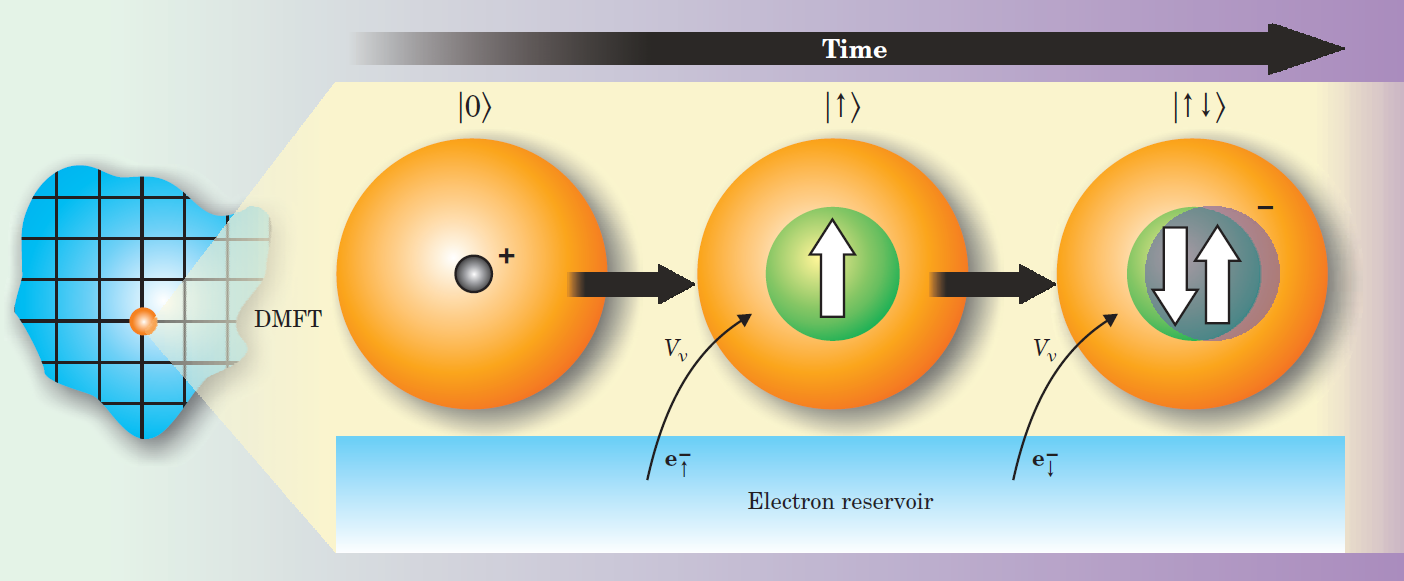
\includegraphics[width=0.8\textwidth]{qips.png}
      \vspace{-10pt}
        \caption{G. Kotliar and D. Vollhardt, Phys. Today March, 53 (2004)}
    \end{center}
  \end{figure}
\vspace{-20pt}
\begin{itemize}
 \item Quantum Impurity Problems(QIPs) were initially constructed to describe the quantum mechanical 
       properties of an impurity or imperfection such as 
       a magnetic atom, dislocation, or a substitutional ion in a lattice.
 \item Many-body lattice problems, such as heavy fermion systems, Mott metal-insulator transition, 
       nonconventional superconductivity could be mapped to QIPs with dynamical mean field theory (DMFT).
\end{itemize}
}

\frame { \frametitle{Quantum Impurity Model}
A quantum impurity model may be represented as a Hamiltonian $H_\text{QI}$

\begin{block}{$H_\text{QI}=H_\text{loc}+H_\text{bath}+H_\text{hyb}$}
\begin{eqnarray}
H_\text{loc}&=& H_\text{loc}^0+H_\text{loc}^I= \sum_{ab} E^{ab}d^\dagger_a d_b + \sum_{pqrs}I^{pqrs}d^\dagger_p d^\dagger_q d_r d_s \\
H_\text{bath}&=&\sum_{k\alpha} \varepsilon_{k\alpha}c^\dagger_{k\alpha}c_{k\alpha} \\
H_\text{hyb}&=&\sum_{k\alpha b} ({V}_k^{\alpha b}c^\dagger_{k\alpha}d_b +\text{h.c.})
\end{eqnarray}
\end{block}
$H_\text{loc}$ describes the ``impurity'' (a system
with a finite (typically small) number of degrees of freedom), 
$H_\text{bath}$ describes the noninteracting system, 
and $H_\text{hyb}$ gives the coupling between the impurity and bath.
}

\frame { \frametitle{Anderson Impurity Model}
The Anderson impurity model describes a localized electronic level, subject to a local Coulomb interaction, which
is coupled to a band of non-interacting conduction electrons.
In the  single-impurity single-orbital case, its Hamiltonian reads
\begin{block}{}

\begin{eqnarray}
H_\text{AIM}&=& \underbrace{\sum_{k\sigma}\varepsilon_k c^\dagger_{k\sigma}c_{k\sigma}}_{H_\text{bath}} 
             +  \underbrace{\sum_\sigma \varepsilon_0d^\dagger_\sigma d_\sigma +Un_\uparrow n_\downarrow}_{H_\text{loc}}\nonumber \\
            &+& \underbrace{\sum_{k\sigma}\Big(V_kc^\dagger_{k\sigma}d_\sigma+h.c.\Big)}_{H_\text{hyb}}
\end{eqnarray}

$\varepsilon_0$ is the level energy and $Un_\uparrow n_\downarrow$ is the interaction term.

\end{block}
}
